\documentclass{article}
\usepackage{styles/project_style} % Assuming you have this style file
\addbibresource{references/projects.bib}

% --- TITLE PAGE INFORMATION ---
\title{Introduction to the Allee effects}

\begin{document}
\maketitle

\section{Agent-Based Models}

Agent-based models (ABMs) are computer simulations used to understand how individual behaviors and interactions give rise to outcomes at the population level. In epidemiology, ABMs are particularly useful for simulating how diseases spread through a population, based on the actions and characteristics of individuals.

In an ABM, each person is represented as an \emph{agent}. Agents are assigned attributes such as age, vaccination status, health condition, or mobility. They follow rules that describe how they behave, interact with other agents, and respond to changes in their environment. Unlike compartmental models, which group individuals into categories (such as susceptible, infected, or recovered), ABMs simulate each individual separately. This allows for more detailed modeling of variation between people.

\begin{figure}[htbp]
  \centering
  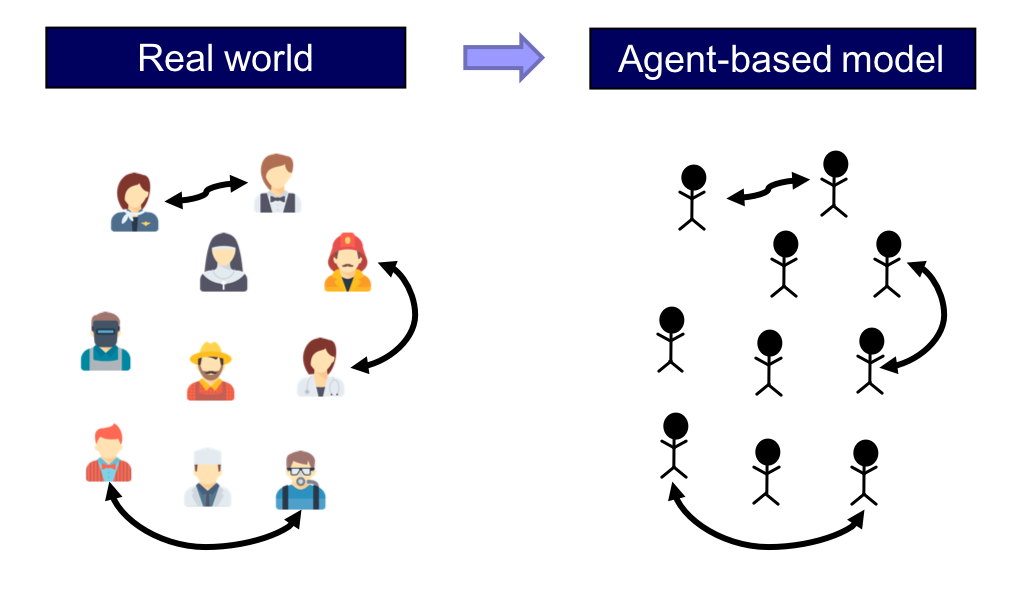
\includegraphics[width=0.7\textwidth]{projects/agent_based_modeling/images/agent-based-modelling.png}
  \caption{Illustration of the agent based modeling concept. Agent-based simulation model is a set of interacting objects that reflect relationships in the real world. The agent-based modeling approach the focus is directly on individual objects, their behavior, and their interaction.}
  \label{fig:allee-effects}
\end{figure}

ABMs are \emph{bottom-up} models: instead of starting with a population average, they build complex outcomes from simple individual behaviors. These behaviors and interactions can lead to \emph{emergent effects}---patterns at the group level that are not obvious from the behavior of individuals alone.

One major strength of ABMs is their ability to simulate systems where:
\begin{itemize}
    \item Individuals are not independent (e.g., household or social network transmission),
    \item Feedback loops exist (e.g., people changing behavior in response to disease prevalence),
    \item Hypothetical or counterfactual scenarios are of interest (e.g., the effects of interventions that haven't yet occurred or cannot be tested in the real world).
\end{itemize}

Because agents operate independently, ABMs can easily include structured contact networks (such as families, schools, or workplaces) and individual-level interventions (such as contact tracing or targeted vaccination). They can also track details such as who infected whom and how infection paths develop through a network.

ABMs are typically \emph{stochastic}, meaning that randomness is built into the simulation. Each run may produce slightly different outcomes, so it is common practice to run the model many times and examine the distribution of results.

Despite their flexibility, ABMs have several limitations:
\begin{itemize}
    \item They can be computationally intensive and more complex to implement than simpler models.
    \item They often require detailed data on individual behavior and disease parameters, which may be unavailable or difficult to estimate.
    \item Because they can model scenarios that have not occurred, it can be difficult to validate the results against real-world observations.
\end{itemize}

Overall, ABMs provide a powerful tool for exploring how individual-level differences and interactions influence system-wide outcomes. They are particularly valuable when studying dynamic, interrelated processes involving feedback, social structure, or behavior change, and when real-world experimentation is not feasible.

\section{Comparison with Differential Equation Models}

Agent-based models (ABMs) and conventional models based on differential equations represent two different approaches to modeling dynamic systems such as disease transmission. Each has its strengths and limitations, and they are suited to different types of questions and data availability.

Traditional models in epidemiology often use systems of ordinary differential equations (ODEs) to describe how the number of individuals in various health states (e.g., susceptible, infected, recovered) changes over time. These are known as \emph{compartmental models}. In these models, individuals are grouped into compartments, and equations specify how people move between compartments based on fixed rates.

\emph{Key differences between ABMs and differential equation models:}
\begin{itemize}
    \item \textbf{Level of abstraction:} ODE models work with aggregate numbers and assume homogeneous mixing within compartments. ABMs simulate individuals and their interactions explicitly.
    
    \item \textbf{Individual heterogeneity:} ODE models assume that all individuals in a compartment are the same. ABMs allow each agent to have unique characteristics (e.g., different behaviors, health risks, or vaccination histories).
    
    \item \textbf{Contact structure:} ODE models typically assume random mixing, meaning that every individual has an equal chance to contact any other. ABMs can include structured networks (e.g., family units, schools) and spatial information.
    
    \item \textbf{Emergent behavior and feedback:} ABMs naturally capture complex interactions and feedback loops (e.g., behavior changes in response to perceived risk). These are difficult to represent in ODE models unless explicitly built into the equations.
    
    \item \textbf{Flexibility and experimentation:} ABMs can simulate counterfactual scenarios or interventions that are difficult or unethical to test in reality. ODE models are more limited in this regard, especially when individual-level mechanisms are important.
    
    \item \textbf{Complexity and computation:} ODE models are usually simpler and computationally efficient. ABMs are more complex to design and require more computational resources, especially when simulating large populations.
    
    \item \textbf{Data requirements:} ODE models can be parameterized with a small number of average values (e.g., average transmission rate). ABMs often require detailed data at the individual or subgroup level to define agent attributes and behaviors.
    
    \item \textbf{Determinism vs. Stochasticity:} Many ODE models are deterministic, producing the same output for the same inputs. ABMs are typically stochastic, meaning results can vary from run to run due to random interactions.
\end{itemize}

In summary, differential equation models are well-suited for understanding average trends in large, relatively homogeneous populations. ABMs, while more complex, are better suited for situations where individual differences, network structures, or behavior change are important to the dynamics being studied. Choosing between the two approaches depends on the modeling goal, data availability, and the desired level of detail.

\section{Implementation Example}
The following code demonstrates an agent-based implementation of the SI (Susceptible–Infected) model in MATLAB. Unlike the equation-based approach shown in the sample, this spatial agent-based model tracks individual agents moving in a two-dimensional space, providing a more granular view of disease spread dynamics.

The model employs a discrete-time, discrete-space approach where agents move randomly on a grid and can infect others when they occupy the same position. This methodology is particularly useful for studying the effects of spatial heterogeneity and stochastic processes on epidemic spread.

The code is structured into four main components: parameter definition, initialization, simulation loop, and movement function. The first part defines the key parameters that govern the model behavior:

\begin{lstlisting}[caption={Parameteres}]
% ----- Parameters -----
area = 100;
population = 1000;
initial_infected = 1;
iterations = 1500;
infection_probability = 0.5;
\end{lstlisting}

Here, area defines the dimensions of the square spatial domain (100×100 units), population represents the total number of agents, and \texttt{initial\_infected} sets the number of agents that start in the infected state. The iterations parameter determines the simulation duration, while \texttt{infection\_probability} represents the likelihood of disease transmission when a susceptible agent encounters an infected one.
The initialization section prepares the simulation environment:
\begin{lstlisting}[caption={Initialization}]
% ----- Initialization -----
position = randi(area, population, 2);      % Random positions
status = ones(population, 1);               % 1 = Susceptible
status(1:initial_infected) = 2;             % 2 = Infected

infected_count    = zeros(iterations,1);
susceptible_count = zeros(iterations,1);

 %----- Prepare plotting  -----
figure(1); 
set(gcf, 'Position', [100, 100, 1200, 500]);
tiledlayout(1, 2);

\end{lstlisting}

Each agent is assigned a random position within the defined area and initially set as susceptible (\texttt{status = 1}), except for a predefined number of infected agents (\texttt{status = 2}). Arrays are preallocated to track the number of susceptible and infected individuals over time, optimizing computational efficiency.
The visualization setup creates a figure with two side-by-side plots:

The core simulation loop performs four key operations at each time step:

\begin{lstlisting}[caption={Simulation loop}]
for i = 1:iterations
    % ----- Infection logic -----
    for person = 1:population
        if status(person) == 1
            same_x = position(:,1) == position(person,1);
            same_y = position(:,2) == position(person,2);
            nearby_infected = same_x & same_y & (status == 2);
            if any(nearby_infected) && rand < infection_probability
                status(person) = 2;
            end
        end
    end

    % ----- Record counts -----
    susceptible_count(i) = sum(status == 1);
    infected_count(i)    = sum(status == 2);

    % ----- Plot  -----
    nexttile(1); cla;
    hold on;
    plot(position(status==1,1), position(status==1,2), 'go', 'MarkerFaceColor','g');
    plot(position(status==2,1), position(status==2,2), 'ro', 'MarkerFaceColor','r');
    axis square; xlim([0 area]); ylim([0 area]);

    nexttile(2); cla;
    plot(1:i, susceptible_count(1:i), 'g', 'LineWidth', 2); hold on;
    plot(1:i, infected_count(1:i), 'r', 'LineWidth', 2);
    title('S vs. I over time'); xlim([1 iterations]); ylim([0 population]);
    drawnow;

    % ----- Move agents -----
    for p = 1:population
        [x, y] = move(position(p,1), position(p,2), area);
        position(p,:) = [x, y];
    end
end
\end{lstlisting}

First, the infection logic checks each susceptible agent to determine if they occupy the same position as any infected agent. If so, transmission occurs with probability \texttt{infection\_probability}. This stochastic element adds realism to the model by acknowledging that not all contacts result in infection. Second, the model records the current counts of susceptible and infected individuals for later analysis.

Third, the visualization component creates two plots that update in real-time: a spatial representation showing agent positions and disease states (green for susceptible, red for infected), and a time series showing the evolution of both populations over time.
Finally, agents move randomly to adjacent positions according to the defined movement function:

\begin{lstlisting}[caption={Move function)}]
function [x, y] = move(x, y, area)
    switch randi(4)
        case 1, if y < area, y = y + 1; end  % up
        case 2, if y > 1,    y = y - 1; end  % down
        case 3, if x > 1,    x = x - 1; end  % left
        case 4, if x < area, x = x + 1; end  % right
    end
end
\end{lstlisting}

This function implements a simple random walk where agents can move in one of four cardinal directions (up, down, left, or right) with equal probability, while ensuring they remain within the boundaries of the simulation area.
Unlike the differential equation-based model in the sample, this agent-based approach captures the spatial heterogeneity of disease spread and allows for the emergence of complex patterns from simple individual-level rules. It provides insights into how spatial clustering affects transmission dynamics and how stochastic events can influence epidemic trajectories. Such models are particularly valuable for studying localized outbreaks, the effects of population density, and interventions that have spatial components (e.g., movement restrictions).

For more complex scenarios, this model could be extended to include additional compartments (such as Exposed or Recovered states), variable movement patterns, or heterogeneous transmission probabilities based on individual characteristics or environmental factors.

\section{Literature}
\subsection{General introduction}
The topic is well discussed in several online resources. Wikipedia is a good starting point. There are many videos on YouTube on the topic. See:
\begin{itemize}
    \item \textcite{AgentBasedModel_Wiki}
    \item \textcite{AgentBasedModel_Macal2010}
    \item \textcite{AgentBasedModel_Macal2014}
    \item \textcite{AgentBasedModel_Sayama}
\end{itemize}

\subsection{Journal Club}
Allee effect is extensively used in population modeling. Here are several papers that can be discussed in the Journal Club presentation.
\begin{itemize}
    \item \textcite{AgentBasedModel_Ciunkiewicz2022} 
    \item \textcite{AgentBasedModel_Hunter2018}
    \item \textcite{AgentBasedModel_Nitzsche2024}
        \item \textcite{AgentBasedModel_Perez2009}
\end{itemize}



\printbibliography

\end{document}